% id: 207-480
% book: 개념원리 대수 · 22 코사인법칙
% section: 연습문제 STEP 2
% figure: crop:fig-207-480.png
% answer: $10\sqrt{6}\mkern3mu \mathrm{m}$
% answer_source: 답지
% variant_level: 0 (원본 전사)
% 이 파일은 build.mjs 가 items.json 에서 만든다. 고칠 때는 items.json 을 고친다.
\smash{\raisebox{1.5mm}{\dmkichul{개념원리 대수 207쪽 480번}}}
\noindent\begin{minipage}[t]{0.58\linewidth}\vspace{0pt}\raggedright 오른쪽 그림과 같이 $40\mkern3mu \mathrm{m}$ 떨어진 지평면의 두 지점~$\pt{A}$, $\pt{B}$에서 하늘 위의 한 지점~$\pt{P}$에 떠 있는 드론을 보았다. $\angle\pt{PAB}=75^\circ$, $\angle\pt{PBA}=60^\circ$, $\angle\pt{PAQ}=30^\circ$일 때, 드론의 높이를 구하시오.\end{minipage}\hfill\begin{minipage}[t]{0.4\linewidth}\vspace{0pt}\centering \setlength{\dmfigw}{92.0pt}\ifdim\dmfigw>\linewidth\setlength{\dmfigw}{\linewidth}\fi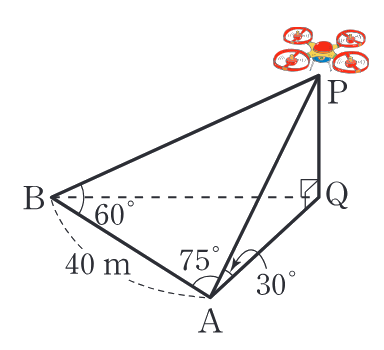
\includegraphics[width=\dmfigw]{figures/fig-207-480.png}\end{minipage}\par
